\documentclass[a4paper]{scrreprt}

\usepackage{scrhack}
\usepackage{graphicx}
\usepackage[utf8]{inputenc}

\addtokomafont{titlehead}{\flushright}
\addtokomafont{subject}{\vspace{3cm}\flushleft}
\addtokomafont{title}{\flushleft}
\addtokomafont{subtitle}{\flushleft}
\addtokomafont{author}{\flushleft\setlength{\tabcolsep}{0pt}}
\addtokomafont{date}{\flushleft}
\addtokomafont{publishers}{\flushleft}

\titlehead{
\includegraphics[scale=2]{logo_en}}
\subject{Software Engineering and Design}
\title{Design Thinking}
\subtitle{Mental Health Care Patient Management System (MHC-PMS)}
\author{
\begin{tabular}{l}
\normalfont\bfseries{Team White:}\\
Dellsperger Jan\\
Ellenberger Roger\\
Sheppard David\\
Sidler Matthias\\
Spring Mathias\\
Thöni Stefan
\end{tabular}
}
\date{\today}
\publishers{Version 1.0}

\begin{document}

\begin{titlepage}
	\maketitle
\end{titlepage}



\section*{Über dieses Dokument}
Dieses Dokument beschreibt den Design Thinking Prozess von \textit{Team White}. Das Dokument beschreibt die Erkenntnisse der einzelnen Schritte über mehrere Iterationen hinweg.


\chapter{Prozess-Ablauf}
\section*{16.03.2016}
\paragraph{Research}
Vor dem eigentlichen Scoping hat jedes Teammitglied unabhängig 15 Minuten recherchiert. So fanden wir heraus, welche Fragen offen sind, welche Zielpersonen die Software zukünftig brauchen könnten und evtl. auch bereits erste Probleme die zu lösen sind.


\paragraph{Scoping}
Auf Basis der ersten Erkenntnisse führten wir das erste Scoping durch.


\paragraph{Research}
In einer zweiten Analyse recherchierten alle Teammitglieder nach Domänen-Wissen zu psychiatrischer Betreuung, Konkurrenzprodukten und möglichen Nutzern.


\paragraph{Scoping}
Scoping erweitert. Die Haupt-Frage ist, ob unsere Benutzergruppe noch mehr Anforderungen hat als ein gutes Reporting. Hierzu wollen wir in weiteren Recherchephasen mehr herausfinden. Zudem suchten wir schon etwas spezifischer welche Reports und Statistiken ein Benutzer der Software brauchen könnte.


\paragraph{Syntesis}
Erste Personas erstellt. Mehrere davon auf Anhieb verworfen.


\paragraph{Design}
Jederes Teammitglied hatte 15 Minuten Zeit um Storybaords zu erstellen. Die Ergebnisse wurden diskutiert. Wir wissen immer noch zu wenig genau, was der User braucht.

\paragraph{Research}
Jedes Teammitglied betreibt individuelle Research als "Hausaufgabe" (je nach verfügbarer Zeit).




\section*{18.03.2016}
\paragraph{Design}
Weitere Storyboards entwickelt


\paragraph{Prototype}
30 Minuten Prototyping (jeder individuell) und verglichen, Ideen gesammelt. Grosse Unterschiede zwischen den einzelnen Prototypen, da jedes Teammitglied andere Vorstellungen des Endprodukts hat.


\paragraph{Syntesis}
Erkenntnisse aus Prototypen in Anforderungsanalyse zusammengetragen.


\paragraph{Research}
Interviewfragen vorbereitet



\section*{22.03.2016}
\paragraph{Research}
Vorbereiten der Interviews.


\section*{23.03.2016}
\paragraph{Research}
Interview mit Mitarbeiten aus dem Managements eines Spitals und einer Klinik.


\section*{24.03.2016}
\paragraph{Research}
Interview mit einer Abteilungsleiterin einer Pflegestätte. Anschliessendes auswerten der Informationen.



\section*{25.03.2016}
\paragraph{Syntesis}
Verarbeiten der Interviewinformationen, definieren der Main-Features. Review und finale Definition der Personas.

\paragraph{Design}
Definieren neuer Storyboards.


\paragraph{Prototype}







\chapter{Ergebnisse}
\section{Scoping}

\subsection{Vorgaben}
Die Hauptzielgruppe für die Software ist vorgegeben: Manager.

\bigskip


\textbf{Fragen (aufgetaucht in Diskussion):}
\begin{itemize}
\item Welche Personen gehören zu unserer Zielgruppe? (Charakter, sozialer Status, Alter, Geschlecht, Ausbildungsniveau, etc.)
\item In wie fern unterscheiden sich die Leute in unserer Zielgruppe? Haben einige Personen deutlich abweichende Anforderungen als andere?
\item Was sind die Hauptfragen des Managements, welche die Software helfen soll zu beantworten?
\item Welche Institutionen werden die Software verwenden? (Spitäler, Krankenkassen, Bundesämter...)
\item Welche rechtlichen Grundlagen muss die Lösung erfüllen?
\end{itemize}


\textbf{Fragen zum Alltag des Benutzers:}

\begin{itemize}
\item Welche Einblicke / Ergebnisse (aus den gesammelten Daten) braucht der Benutzer?
\item Welche Probleme hat der Benutzer?
\item Welchen Hintergrund hat der Benutzer? (Karriere, Leistungsausweis, Informatikkenntnisse)
\item Gibt es Benutzer die oft repetitive Tätigkeiten ausführen?
\item In welche Position arbeitet der Benutzer?
\end{itemize}

\textbf{Themen ausserhalb unseres Aufgabenbereichs:}

\begin{itemize}
\item Anforderungen die explizit nicht nicht mit \textit{Metal Health} zusammenhängt
\item Bedürfnisse von Benutzern aus der Administration (Rechnungsstellung, Patientenverwaltung, etc.)
\end{itemize}



\section{Research}
\paragraph{Recherche-Vorgehen:} 
\begin{itemize}
\item Internet-Recherche
\item Interviews
\end{itemize}


\paragraph{Recherchethemen:} 
\begin{itemize}
\item Benutzer-Rollen
\item Grundlegende Probleme in Healt-IT (Stichwörter: ACM CHI, Health IT (HIT), Useability in HIT)
\item Lösungen von Konkurrenten
\item Rechtliche Grundlagen
\end{itemize}

\subsection{Benutzer-Rollen}
Zum einen haben wir hierzu Personen in Kaderpositionen in Gesundheitswesen gesucht (via xing, LinkedIn) 




\paragraph{Anforderungen der Benutzer}
Ablegen der Gesundheitshistorie mit Tags


\subsection{Probleme in Health-IT}
\paragraph{Patientensicherheit} In Health IT ist eines der grössten Probleme die Patientensicherheit. Viele Anbieter sind besorgt, dass ein Softwarefehler Leben kosten kann. Zudem ist es schwer eine Balance zwischen Benutzerfreundlicher Bedienung und Sicherheit zu finden.\footnote{http://interactions.acm.org/archive/view/july-august-2012/measuring-usability-in-healthcare-it}
Für unsere Zielgruppe ist dieser Punkt aber weniger von Bedeutung.

\paragraph{Heterogene IT Systeme} Health IT ist ein sehr komplexes Themengebiet, da die zusammenarbeitenden Systeme sehr heterogen sind. \footnote{Informationen aus Interview vom 23.03.2016}



\subsection{Konkurrenzprodukte}
\paragraph{Insights} Eine Anforderung an die Software ist, durch gutes Reporting Einblicke zu erhalten, die vorher nicht so einfach oder gar nicht möglich waren. Das Oberthema dazu ist \textit{Analytics} und \textit{Business Intelligence}. Ein bekanntes Produkt in diesem Bereich ist Microsoft PowerBI\footnote{https://powerbi.microsoft.com/en-us/} .

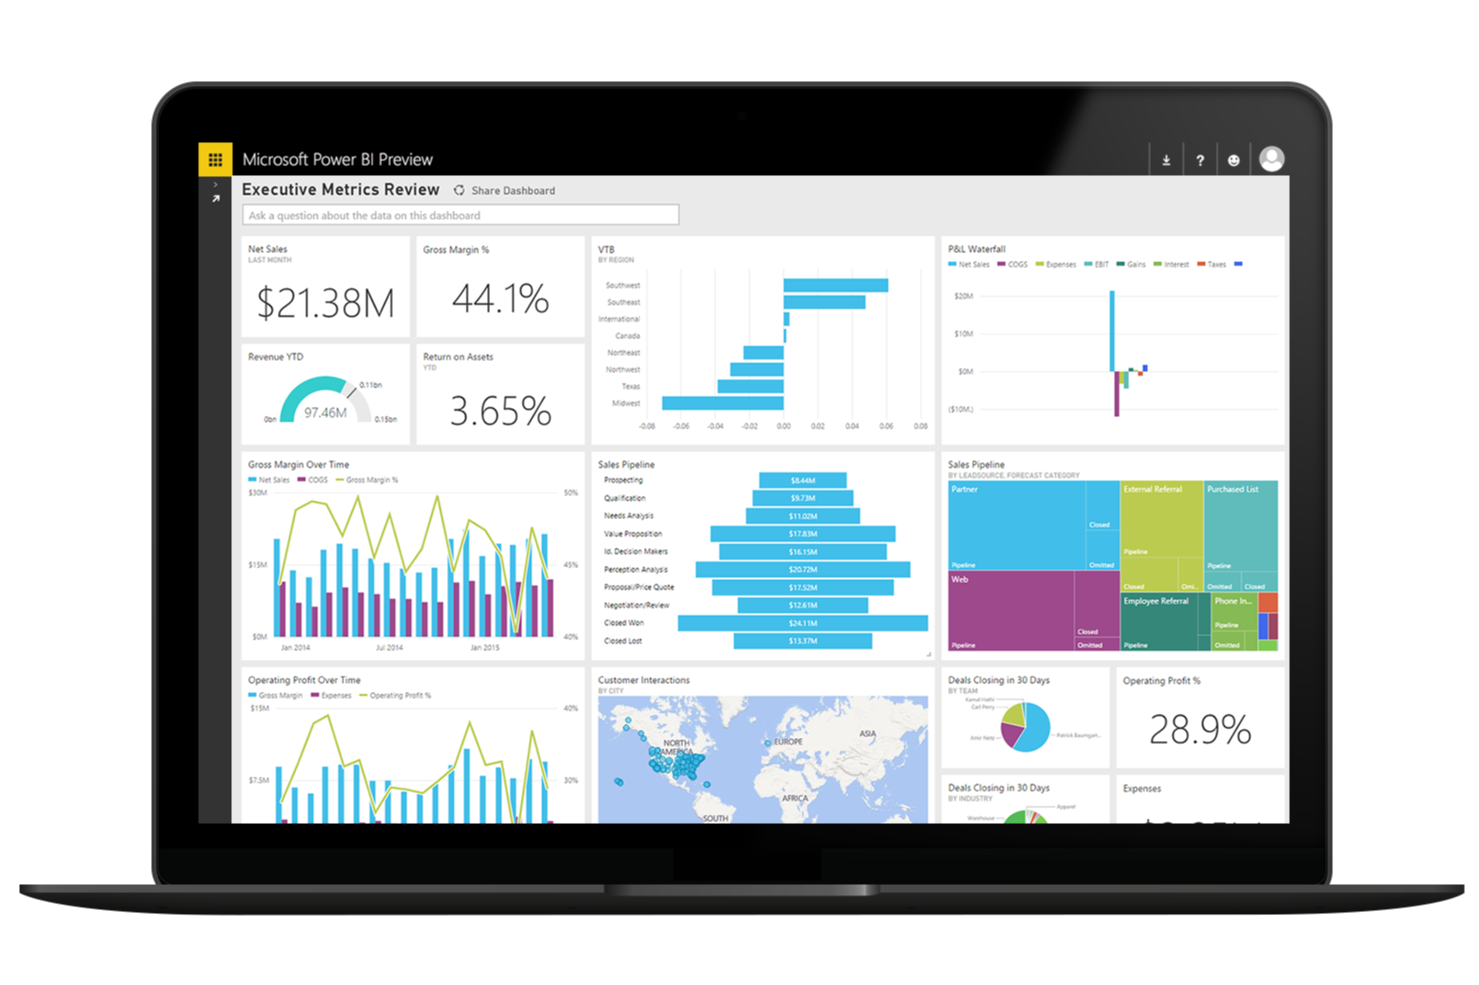
\includegraphics[width=0.6\textwidth]{img/research_ms-powerbi.png}

Microsoft bietet hier ein Werkzeug mit dem sich bereits gesammelte Daten effektiv analysieren und visualisieren lassen. Die generierten Berichte lassen sich über einen Webbrowser oder ein Mobiles Endgerät einsehen. Der Dienst läuft in der Cloud ist daher nicht geeignet für das direkte Verarbeiten von Patientendaten.

\bigskip

Das Schweizer Unternehmen \textit{Erne Consulting} bietet für ihre eHealth-Lösung Polypoint für diesen Zweck eine Reporting-Erweiterung an \footnote{http://polypoint.ch/}.

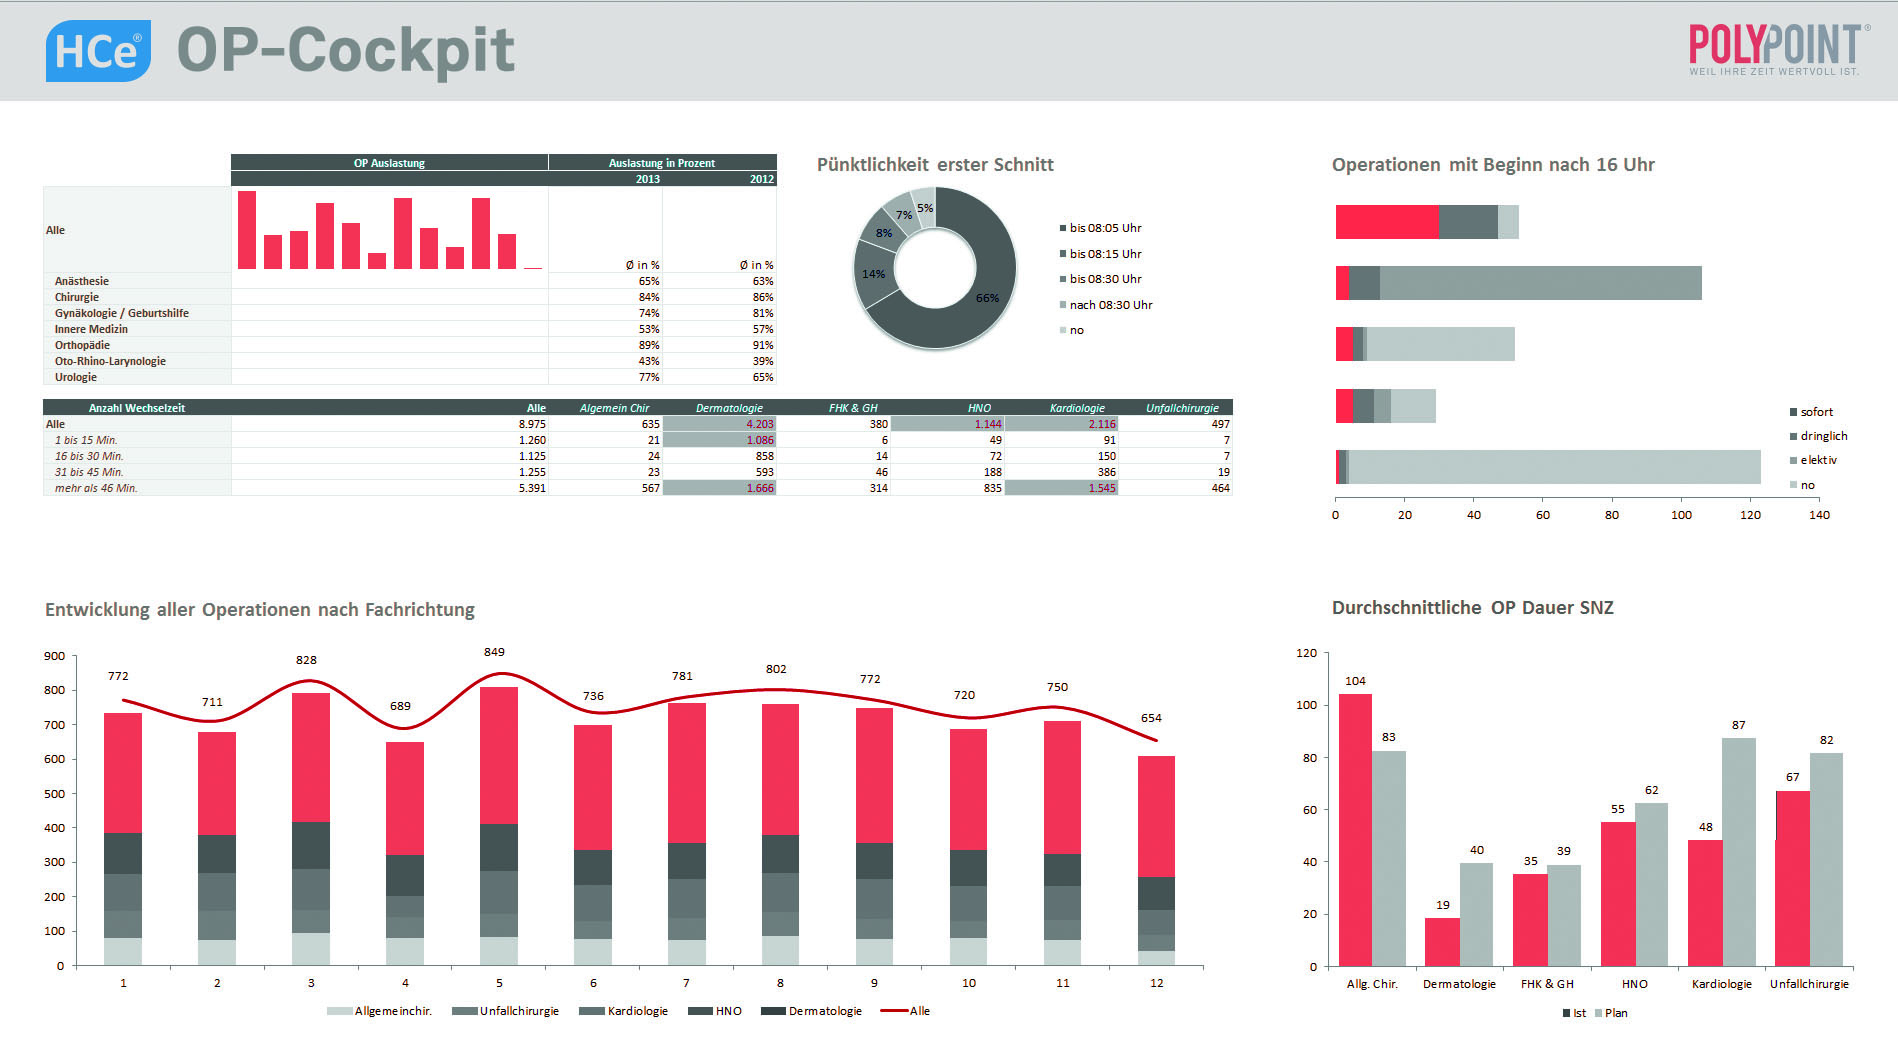
\includegraphics[width=0.9\textwidth]{img/research_polypoint_op-cockpit.jpg}



\subsection{Rechtliche Grundlagen}
TODO: Rechtliche Grundlagen abklären

Mental Health Act

Datenschutz: BEKIS Plus





\section{Syntesis}
Gerade in den Interviews wurde ersichtlich, dass die Zielgruppe Manager mehr eine Rolle ist, als eine konkrete Person. Je nach Grösse der Betreuungseinrichtung gibt es keinen expliziten Manager. In kleineren Einrichtungen hat auch ein Arzt die Rolle Manager inne.
Die Anforderungen gehen je nach Grösse des Zielkunden auseinander.

Aus den gewonnen Erkenntnissen der Recherche-Phase haben wir einige mögliche Personas erstellt:

\paragraph{Ariane} leitet die Abteilung Pflege in einer grossen Betreuungseinrichtung für Personen mit psychischen Störungen. Damit übernimmt Sie die Personalplanung und ist verantwortlich, dass die Prozesse in der Einrichtung funktionieren. Aufgrund ihrer grossen Führungsspanne arbeitet sie sehr strukturiert und sucht stets Möglichkeiten Zeit zu sparen.

Sie will zudem stets informiert sein über aktuelle Notfälle oder sonderbare Ereignisse im Zusammenhang mit den Patienten. Sie will stets die Hintergründe kennen, warum etwas passiert und überlässt nichts dem Zufall.


\paragraph{Bruno} ist leitender Arzt einer kleinen Betreuungseinrichtung für ambulante Behandlung von Personen mit psychischen Störungen. Er leitet die Praxis alleine. Unterstützend für die Behandlung, den Empfang und die Büroarbeit arbeiten zwei Assistentinnen unter seiner Führung. Der Umgang untereinander ist sehr familiär und basiert auf erwähnenswert viel Vertrauen.


\section{Design}
TODO: Storyboards noch einbinden


\section{Prototype}
TODO: Prototypen einbinden.


\section{Validate}
TODO: Prototypen validieren.






\end{document}